% 2020 全国Ⅱ卷 理20：三棱柱 ABC-A1B1C1 及截面四边形 EB1C1F
% 来源 PDF：普通高考/2020/2020全国2理(…).pdf 第 2 页（A3 横排），印面 1122，第 20 题题干下方
% 结构：底面 ABC 为正三角形，侧面 BB1C1C 为矩形（BB1⊥BC）；M、N 为 BC、B1C1 的中点，
%       O 为 △A1B1C1 的中心，P 在 AM 上，截面 EB1C1F 与底面交于 EF（EF∥BC）。
%       实线：A1A、A1B1、A1C1、B1C1、C1C、CB、BA、B1B、NM、B1E；
%       虚线：AC、AO、EF、FC1（均被棱柱本身遮挡）。
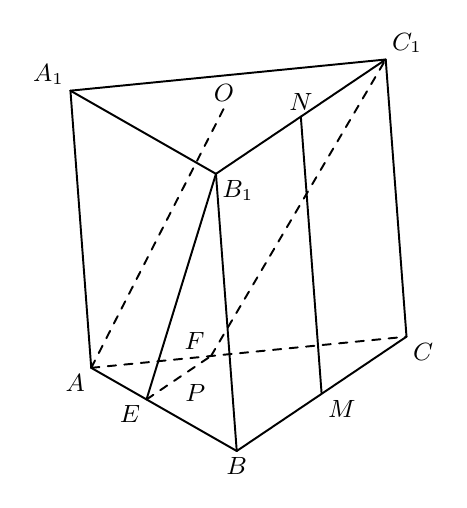
\begin{tikzpicture}[line width=0.7pt, font=\small,
  x=0.88cm, y=0.88cm, line cap=round, line join=round]
  % 底面 ABC 与上底面 A1B1C1 的平行投影
  \coordinate (A)  at (1.75,1.20);
  \coordinate (B)  at (3.85,0.00);
  \coordinate (C)  at (6.30,1.65);
  \coordinate (A1) at (1.45,5.20);
  \coordinate (B1) at (3.55,4.00);
  \coordinate (C1) at (6.00,5.65);
  % 中点、中心与截面相关点
  \coordinate (M)  at (5.075,0.825);
  \coordinate (N)  at (4.775,4.825);
  \coordinate (O)  at (3.667,4.950);
  \coordinate (P)  at (3.014,1.058);
  \coordinate (E)  at (2.548,0.744);
  \coordinate (F)  at (3.479,1.371);

  % 可见棱
  \draw (A1) -- (A);
  \draw (A1) -- (B1);
  \draw (A1) -- (C1);
  \draw (B1) -- (C1);
  \draw (C1) -- (C);
  \draw (C)  -- (B);
  \draw (B)  -- (A);
  \draw (B1) -- (B);
  % 中位线与截面可见边
  \draw (N) -- (M);
  \draw (B1) -- (E);

  % 被遮挡的棱与内部辅助线
  \draw[dashed] (A) -- (C);
  \draw[dashed] (A) -- (O);
  \draw[dashed] (E) -- (F);
  \draw[dashed] (F) -- (C1);

  % 顶点标注
  \node[above left,  inner sep=2pt] at (A1) {$A_1$};
  \node[below left,  inner sep=2pt] at (A)  {$A$};
  \node[below,       inner sep=2pt] at (B)  {$B$};
  \node[below right, inner sep=2pt] at (C)  {$C$};
  \node[above right, inner sep=2pt] at (C1) {$C_1$};
  \node[below right, inner sep=2pt] at (B1) {$B_1$};
  \node[above,       inner sep=2pt] at (N)  {$N$};
  \node[above,       inner sep=2pt] at (O)  {$O$};
  \node[below right, inner sep=2pt] at (M)  {$M$};
  \node[below left,  inner sep=2pt] at (E)  {$E$};
  \node[above left,  inner sep=2pt] at (F)  {$F$};
  \node[below right, inner sep=2pt] at (P)  {$P$};
\end{tikzpicture}
